\documentclass{article}

% Language setting
% Replace `english' with e.g. `spanish' to change the document language
\usepackage[english]{babel}

% Set page size and margins
% Replace `letterpaper' with `a4paper' for UK/EU standard size
\usepackage[a4paper,top=2cm,bottom=2cm,left=3cm,right=3cm,marginparwidth=1.75cm]{geometry}

% Useful packages
\usepackage{amsmath}
\usepackage{graphicx}
\usepackage[colorlinks=true, allcolors=blue]{hyperref}

\title{Ranking states for phase measurement}
\author{Tien Nguyen Dinh}

\begin{document}
\maketitle

\begin{abstract}
In this note, we consider the measurement of the phase of an electromagnetic field. The \textit{state} of the field is quantized and therefore reresented as a quantum state. The real measurement apparatus is first neglected and assumed to be performing the so-called canonical phase measurement (\texttt{CAN}), which is the current best known method for the phase estimation. The measurement performance is then relaxed to include homodyne detection (\texttt{HOM}) and heterodyne detection (\texttt{HET}). With each method we calculate relevant metrics with respect to different input quantum states to determine the most efficient one. The result is, behold, I won't tell you now. 
\end{abstract}

\section{First we discuss the why}

Why do we care about the phase measurement after all? The phase measurement is one of the element of the hybrid Steane-Knill error correction circuit (See Figure \ref{fig:steane_knill}) \cite{Grimsmo_2020}. The scheme includes three input modes: the data mode is the middle one; both upper and lower modes are ancillary modes. The data mode is an order-$N_1$ RSB code, while the upper ancillary mode is an order $M$ and the lower ancillary mode is an order $N_2$ RSB code. 

We now restrict ourselves to only the yellow part of the hybrid Steane-Knill EC circuit. In the absence of error, i.e. $k=0, \theta=0$, the CROT gate acts as an identity on the data-ancillary subspace for $\varphi=2\pi/MN_1$,
\begin{align}
    \text{CROT}_{MN_1}|\Psi_M\rangle|\Psi_{N_1}\rangle = |\Psi_M\rangle|\Psi_{N_1}\rangle.
\end{align}
To see this, note that $|\Psi_M\rangle =\sum_{k=0}^\infty f_{kM}|kM\rangle$, $|\Psi_{N_1}\rangle=\sum_{\ell=0}^\infty f_{\ell N_1}|\ell N_1\rangle$. Then,
\begin{align}
    \text{CROT}_{MN_1}|\Psi_M\rangle|\Psi_{N_1}\rangle &= |\Psi_M\rangle|\Psi_{N_1}\rangle,\\
    &=\exp\left(\frac{2\pi}{MN_1}\hat{n}\otimes \hat{n}\right)\left(\sum_{k=0}^\infty f_{kM}|kM\rangle\otimes\sum_{\ell=0}^\infty f_{\ell N_1}|\ell N_1\rangle\right),\\
    &=\sum_{k,\ell=0}^{\infty}f_{kM}|kM\rangle \otimes e^{2\pi k\ell}f_{\ell N_1}|\ell N_1\rangle,\\
    &=|\Psi_M\rangle|\Psi_{N_1}\rangle.
\end{align}
However, in the presence of error $\hat{E}_k(\theta)$ on the data mode, the CROT gate propagates a rotation of $R(-2k\pi/MN_1)$ to the upper ancillary mode. To see this, consider
\begin{align}
    \text{CROT}_{M,N_1}\left[\hat{R}(\theta)\hat{a}^k|\Psi_{N_1}\rangle\right]|\Psi_M\rangle &= \text{CROT}_{M,N_1}\left[\sum_{\ell=0}^\infty \tilde{f}_{\ell N_1}e^{i\theta(\ell N_1-k)}|\ell N_1-k\rangle\right]\otimes \sum_{m=0}f_{mM}|mM\rangle,\\
    &=\sum_{\ell, m=0}^\infty\left(\tilde{f}_{\ell N_1}e^{i\theta(\ell N_1-k)}|\ell N_1-k\rangle \otimes f_{mN}e^{{-2k\pi\hat{n}}/{MN_1}}|mM\rangle \right),\\
    &=\hat{E}_k(\theta)|\Psi_{N_1}\rangle \otimes \hat{R}(-2\pi k/MN_1)|\Psi_M\rangle.
\end{align}
Ok. So far so good. We now want to make a phase measurement on the ancillary mode to estimate $k$. After knowing $k$, it's up to the second part of the circuit to do the teleportation protocol to transfer the damaged codeword to the fresh ancilla (lower mode). 

It should be noted that the state $|\Psi_M\rangle$ must either be a state of discrete rotation symmetry of order $N>1$, or no symmetry at all ($N=1$). A state with continuous rotation symmetry would not work, i.e. a sole Fock number state $|n\rangle$. 

To summarize, the reason why is that we want to estimate $k$. We want to estimate $k$ because it gives off information regarding the loss that had happened on the data mode. This information is useful because we can use it for error correction. 

\begin{figure}
\centering
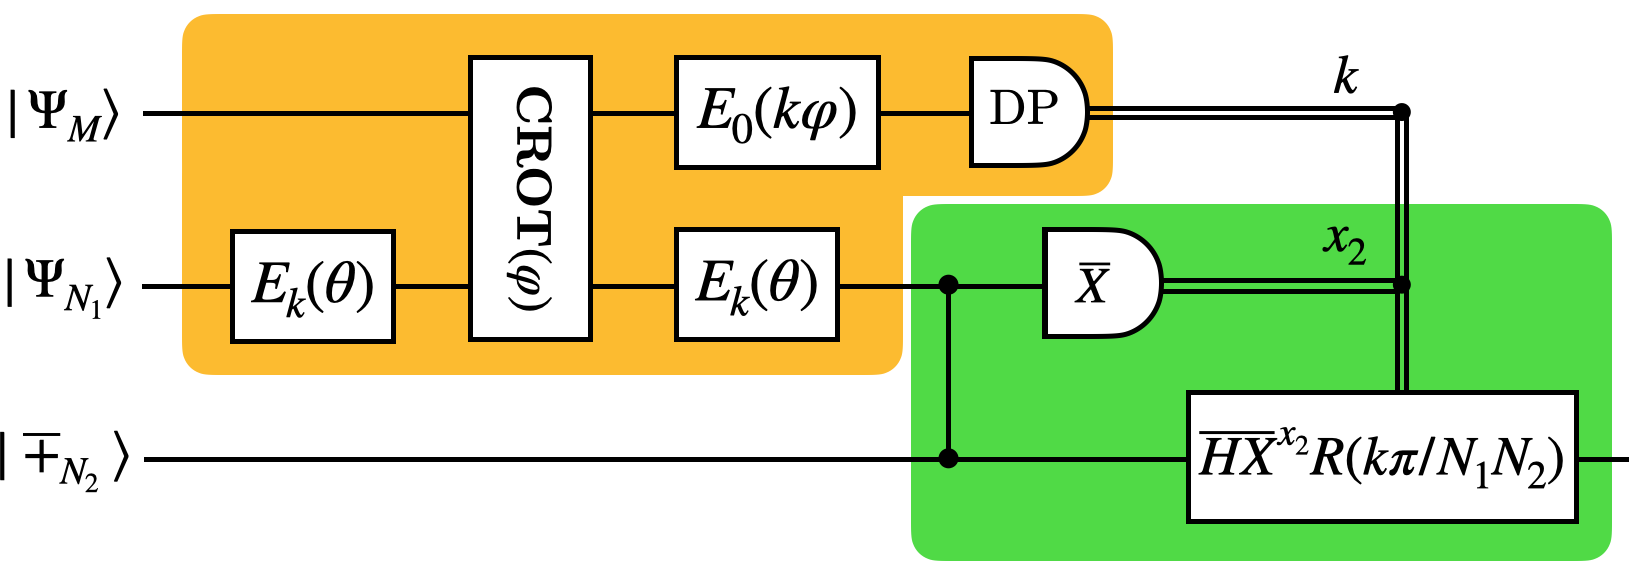
\includegraphics[scale=0.2]{steane_knill.png}
\caption{\label{fig:steane_knill}The hybrid EC gadget: The three modes are the ancillary (upper), data (middle), and output (lower) modes. A CROT gate is applied on the input and ancillary modes, followed by a measurement on the $X$ basis and a discrete phase measurement. A recovery controlled by the classical outcomes $k$ and $x_2$ is finallly applied to the output.}
\end{figure}

\section{Then we discuss the how}
The ``how" here is how good is our guess of $k$. Intuitively, it involves two parties, (a) the input state $|\Psi_M\rangle$ and (b) the discrete phase measurement DP. For what I know, the best discrete phase measurement out there is the canonical phase measurement \texttt{CAN}.

\subsection{\texttt{CAN} and the embedded phase uncertainty}
Let us safely assume that we can perform the \texttt{CAN} phase measurement. Then, the set of POVM elements are
\begin{align}
    \hat{F}^{\texttt{CAN}}(\phi)=\frac{1}{2\pi}|\phi\rangle\langle\phi|,
\end{align}
where $|\phi\rangle$ are the unphysical phase states $|\phi\rangle=\sum_{n=0}^\infty e^{in\phi}|n\rangle$.

One particular metric that we can use to compare different states for the phase measurement being the modular phase uncertainty. \textcolor{blue}{T: I guess this measures how spread the state is in the phase space. Like, for phase state + \texttt{CAN}, this phase uncertainty should be zero--cuz you know, it's perfect, right?} It is defined to be 
\begin{align}
    \Delta_N(\theta)=\dfrac{1}{|\langle e^{iN\theta}\rangle|^2}-1,
\end{align}
wherer the quantity $\langle e^{iN\theta}\rangle $ is the mean modular phase,
\begin{align}
    \langle e^{iN\theta}\rangle = \dfrac{1}{2}\sum_{k=0}^\infty |f_{kN}f_{(k+1)N}|.
\end{align}
The coefficients $f_{kN}$ are the Fock-grid coefficients of the code. 

\section{Phase uncertainty of bosonic rotation symmetric code}

Within this section, we go over through the families of code and compute the embedded phase uncertainty for each. The comparison between them will be presented in the next section.

\subsection{Cat encoding}

Broadly speaking, any thing that starts with coherent states should be associated with cat codes.

\subsubsection{$1$-fold symmetry: A single coherent state}

The coherent state $|\alpha\rangle$ has support on every $n$-th Fock state, therefore it is also can be thought of as a $|+_1\rangle$ state of an order-1 cat code. The state $|\alpha e^{i\pi}\rangle =|-\alpha\rangle$ is the $|-_1\rangle$ state. They are approximately orthogonal (in the limit of large $|\alpha|$). Now, the mean modular phase is 
\begin{align}
    \langle e^{i\theta}\rangle_{\texttt{cat1}} = e^{-|\alpha|^2}\sum_{k=0}^\infty \frac{\alpha^{2k+1}}{\sqrt{k!(k+1)!}}\to 1
\end{align}
as $\alpha\to\infty$. Therefore, the embedded phase uncertainty vanishes for large enough $\alpha$. Figure \ref{fig:compare} shows this. 

\subsubsection{$2$-fold symmetry: Two-legged cat state}

The two-legged cat state is defined as $|\Psi_2\rangle=\mathcal{N}_2(|\alpha\rangle +|-\alpha\rangle)$. It's a state with two-fold rotation symmetry, and therefore would take the operator $\hat{R}_4=\exp[(i\pi/2)\hat{n}]$ as the logical $\bar{Z}$ operator, as a logical plus state of an order-$2$ RSB code $|+_2\rangle$. Now, the mean modular phase is 
\begin{align}
    \langle e^{i2\theta}\rangle_{\texttt{cat2}} = \frac{2e^{-|\alpha|^2}}{1+e^{-2|\alpha|^2}}\sum_{k=0}^\infty \frac{\alpha^{4k+2}}{\sqrt{(2k)!(2k+2)!}}\to 1
\end{align}
as $\alpha\to\infty$. Again, the embedded phase uncertainty vanishes for large enough $\alpha$. Let us plot it on the same plot to compare with the first case (i.e. single coherent state). 

\subsubsection{$3$-fold symmetry: Three-legged cat state}

The three-legged cat state is defined as $|\Psi_3\rangle =\mathcal{N}^\texttt{cat}_3(|\alpha\rangle+|e^{i2\pi/3}\alpha\rangle+|e^{i4\pi/3}\alpha\rangle)$. It's a state with three-fold rotation symmetry, and therefore would take the operator $\hat{R}_{6}=\exp[(i\pi/3)\hat{n}]$ as the logical $\bar{Z}$ operator, as a logical plus state of an order-3 RBS code $|+_3\rangle$. The mean modular phase is 
\begin{align}
    \langle e^{i3\theta}\rangle_{\texttt{cat3}} =\dfrac{3e^{-|\alpha|^2}}{1+2e^{-3|\alpha|^2/2}\cos\left(\sqrt{3}|\alpha|^2/2\right)}\sum_{k=0}^\infty \dfrac{\alpha^{6k+3}}{\sqrt{(3k)!(3k+3)!}}\to 1    
\end{align}
as $\alpha\to\infty$, indeed. Again, the phase uncertainty vanishes in the limit of large $\alpha$. 
\subsubsection{Four-legged cat state}

The four-legged cat state is defined as $|\Psi_4\rangle=\mathcal{N}_4(|\alpha\rangle+|i\alpha\rangle+|-\alpha\rangle+|-i\alpha\rangle)$. It's a state with four-fold rotation symmetry, and therefore would take the operator $\hat{R}_8=\exp[(i\pi/4)\hat{n}]$ as the logical $\bar{Z}$ operator, as a logical plus state of an order-$4$ RSB code $|+_4\rangle$. The mean modular phase is
\begin{align}
    \langle e^{i4\theta}\rangle_{\texttt{cat4}} =\frac{4e^{-|\alpha|^2}}{1+e^{-2\alpha^2}+2e^{-\alpha^2}\cos(\alpha^2)}\sum_{k=0}^\infty\frac{\alpha^{8k+4}}{\sqrt{(4k)!(4k+4)!}}\to 1
\end{align}
as $\alpha\to\infty$, indeed. Again, the embedded phase uncertainty vanishes in the limit of large $\alpha$, albeit slower compared to the single coherent state and the two-legged cat state. 

\subsubsection{Binomial encoding}

Binomial encoding was first introduced in \cite{PhysRevX.6.031006}. The codewords are most straightforwardly defined in the conjugate basis,
\begin{align}
    |+_{N,\texttt{bin}}\rangle = \sum_{k=0}^{K}\left[\dfrac{1}{2^K}\binom{K}{k}\right]^{1/2}|kN\rangle. 
\end{align}
Note that $N$ defines the order of rotation symmetry, and $K$ defines the Fock space truncation. For every $N$, there exists different primitive states with the same order of rotation symmetry. The smallest binomial code is the $N=K=1$ case, as the binomial encoding tends to the trivial encoding, $|+_{1,\texttt{bin}}=(1/\sqrt{2})(|0\rangle+|1\rangle)$. As we keep $K=1$ and increase the symmetry order, $N>1$ we obtain the \texttt{0N} encoding, $|+_{N,\texttt{0N}}\rangle=(1/\sqrt{2})(|0\rangle+|N\rangle)$. Finally, we stress that for a given order of rotation symmetry $N$, we have different binomial encoding for every $K=1,2,\dots$ value.

The average photon number for the binomial encoding is simply $\bar{n}_{\texttt{bin}}=(1/2)NK$. The mean modular phase is 
\begin{align}
    \langle e^{iN\theta}\rangle_{\texttt{bin}N} = \dfrac{1}{2^K}\sum_{k=0}^{K-1}\left[\dfrac{K-k}{k+1}\right]^{1/2}\binom{K}{k}.
\end{align}

\subsubsection{Pegg-Barnett encoding}

A Pegg-Barnett phase state is given by,
\begin{align}
    |\phi, s\rangle = \dfrac{1}{\sqrt{s}}\sum_{n=0}^{s-1}e^{in\phi}|n\rangle. 
\end{align}
where the parameter $s$ sets the truncation level. \textcolor{blue}{Think of a phase state: $|\phi\rangle=\sum_{n=0}^\infty e^{in\phi}|n\rangle$. This kind of state is not normalizable. We then make a truncation to the $s-1$ level to realize a truncated $s$-level Fock space. Then the state is $|\phi\rangle=\sum_{n=0}^{s-1}e^{in\phi}|n\rangle$, which is now normalizable. The normalization constant is nothing but $1/\sqrt{s}$.} We note that for the truncated Fock space of $s$ levels, the set of $|\phi_m\rangle=2\pi m/s, s\rangle$ for $m=0, 1,\dots,s-1$ forms an orthonormal basis. 

The Pegg-Barnett encoding is thus realized using the primitive $|\phi=0, s\rangle$. The truncation $s-1$ must be at least $N$. For an order-1 PB code, $s=2$: this is the trivial encoding $|+_{1,\texttt{pb}}=(1/\sqrt{2})(|0\rangle+|1\rangle)$. \textcolor{red}{Make sure you understand the argument that the PB code, when restricting $s=p\times 2N$ is equivalent to the shift-resistant qudit code}. 

For PB codes, the mean excitation number is $\bar{n}_{\texttt{pb}}= \frac{N}{2}(\lceil s/N \rceil -1)$. The mean modular phase is
\begin{align}
    \langle e^{iN\theta}\rangle_{\texttt{pb}N}=1-\dfrac{1}{\lceil s/N\rceil},
\end{align}
where the function $\lceil x \rceil$ returns the least integer $x$ greater than or equal to $x\in R$. 

\subsection{\texttt{CAN}: A level playing field}
We now level the playing field by comparing states with the \textbf{same} order of rotation symmetry $N$. All states are again taken to be the plus state of an order-$N$ code $|+_{N,\texttt{code}}\rangle$. The primitive state is left to be freely optimized, and only required to have the same number of average excitation number $\bar{n}$. 

Based on the primitives, we broadly have four family of codes: \texttt{cat} codes with the primitive state as the coherent state; \texttt{bin}omial codes with the primitive state as that weird shit state (\textcolor{red}{Make sense of the primitive state of the binomial encoding}); \texttt{pb} codes with the primitive state being the Pegg-Barnett phase state; and finally \texttt{lazy} codes with the primitive state being the lazy state. 

\begin{figure}
\centering
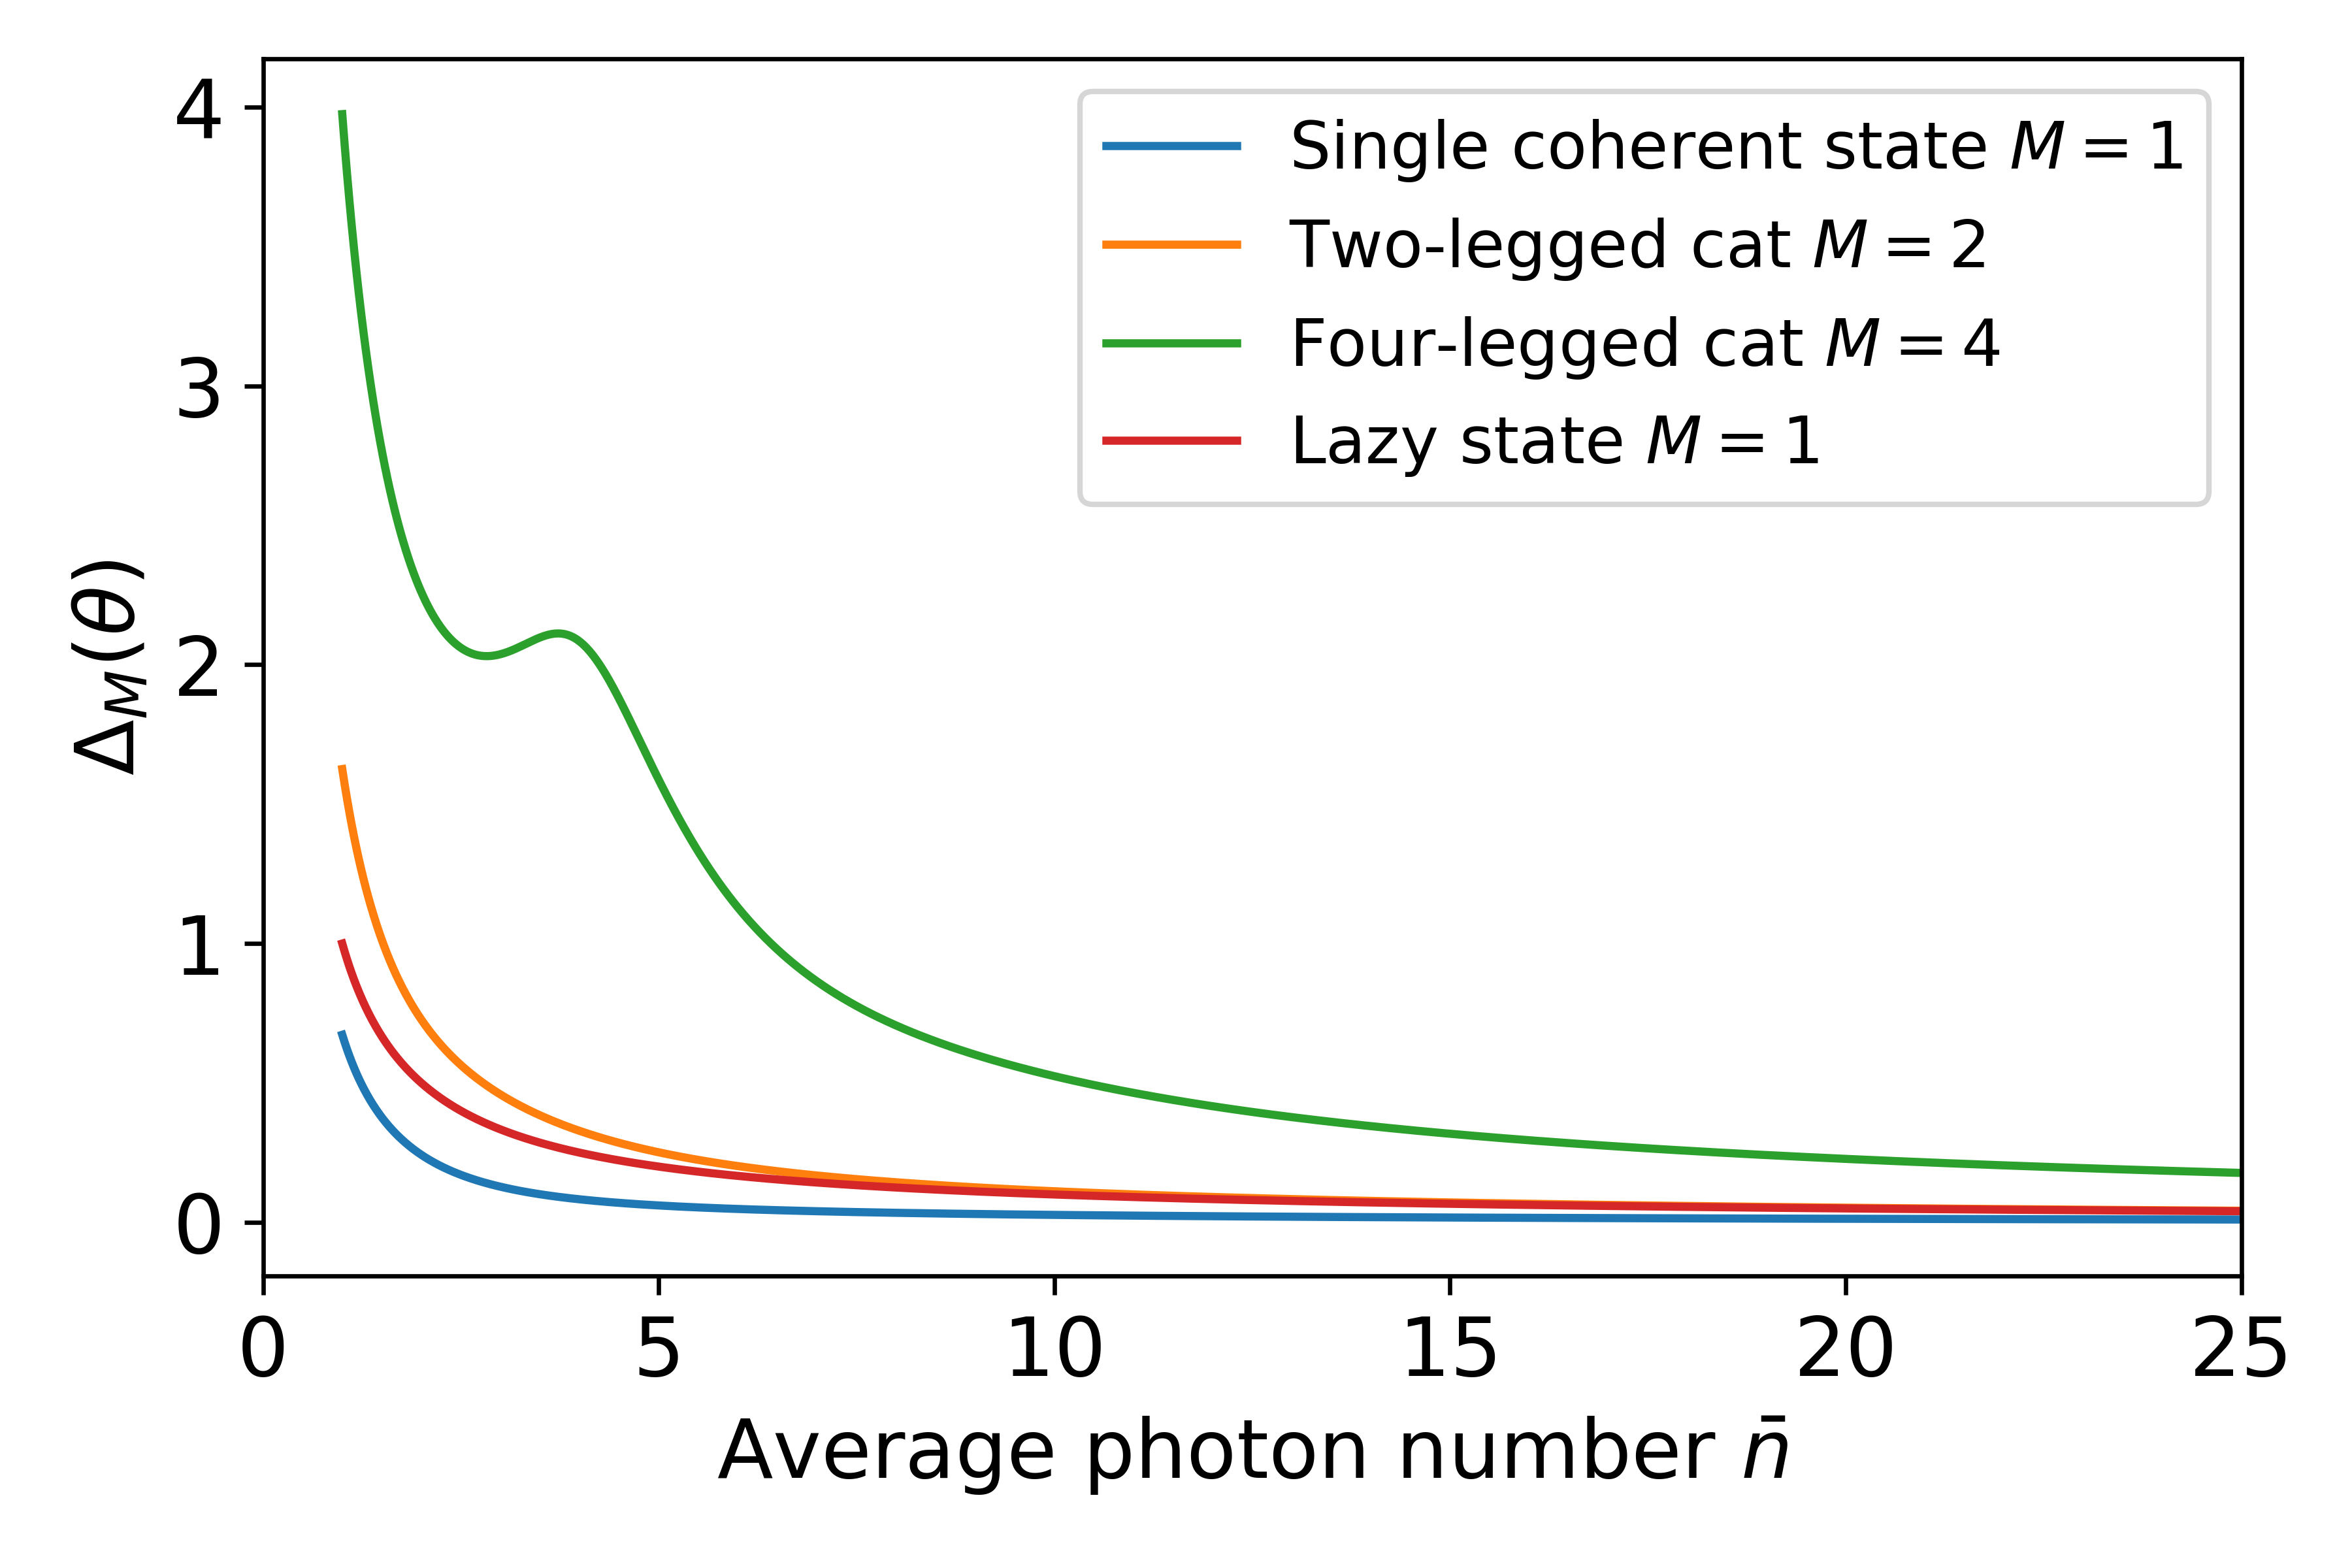
\includegraphics[width=1\linewidth]{compare.png}
\caption{\label{fig:compare}Comparison of the embedded phase uncertainty (EPU) for each cases: a single coherent state, two-legged cat state, four-legged cat state, and the lazy state. For the first three cases where the primitive state being a simple coherent state, the EPUs vanishes in the limit of $\alpha\to\infty$. Meanwhile, the lazy state asymptotes this regime when $b\to 1^+$.}
\end{figure}

\section{Check whether if all these weird cases work: $|N\rangle+|\alpha\rangle$}

\newpage
\appendix
\section{Stuff with coherent states}
\subsection{Normalization for order-2 and order-4 cat codes}
Let $|\alpha e^{i\theta}\rangle$ and $|\beta e^{i\phi}\rangle$ be two coherent states, the inner product of them is
\begin{align}
    \langle \beta e^{i\phi}|\alpha e^{i\theta}\rangle &= e^{-(|\beta|^2+|\alpha|^2)/2}\sum_{k=0}^\infty \frac{\beta^k\alpha^k}{k!}e^{i(\theta-\phi)k},\\
    &=e^{-(|\beta|^2+|\alpha|^2)/2}\sum_{k=0}^\infty \frac{(\beta e^{-i\phi}\alpha e^{i\theta})^k}{k!},\\
    &=e^{-(|\beta|^2+|\alpha|^2)/2}\sum_{k=0}^\infty \frac{(\beta^\ast\alpha)^k}{k!},\\
    &=\exp\left(-\frac{|\beta|^2}{2}-\frac{|\alpha|^2}{2}+\beta^*\alpha\right)
\end{align}
Using this, it follows immediately that $\langle \alpha|-\alpha\rangle = e^{-2|\alpha|^2}$. Thus the normalization constants of the state $|\Psi_2\rangle = \mathcal{N}_2(|\alpha\rangle \pm |-\alpha\rangle)$ are
\begin{align}
    \mathcal{N}^\texttt{cat}_2 = [2(1\pm e^{-2|\alpha|^2})]^{-1/2}.
\end{align}
The normalization constant of the state $|\Psi_4\rangle=\mathcal{N}_4(|\alpha\rangle+|i\alpha\rangle+|-\alpha\rangle+|-i\alpha\rangle)$ is
\begin{align}
    \mathcal{N}^\texttt{cat}_4 = \left[4(1+2e^{-\alpha^2}\cos(\alpha^2)+e^{-2\alpha^2}\right]^{-1/2}.
\end{align}
And finally the normalization for the state $|+_{3,\texttt{cat}}\rangle$ is 
\begin{align}
    \mathcal{N}^\texttt{cat}_3 = \left[3\left(1+2e^{-3|\alpha|^2/2}\cos\left(\sqrt{3}|\alpha|^2/2\right)\right)\right]^{-1/2}.
\end{align}
\subsection{Photon number of superposed coherent states}
First we acknowledge that $\langle \alpha|\hat{n}|\beta\rangle=\exp[-(|\alpha|^2+|\beta|^2)/2]\alpha^*\beta \exp(\alpha^*\beta)$. Then it comes natural that for $|+_2\rangle = \mathcal{N}_2(|\alpha\rangle+|-\alpha\rangle)$ and $|+_4\rangle=\mathcal{N}_4(|\alpha\rangle+|i\alpha\rangle+|-\alpha\rangle+|-i\alpha\rangle)$, the average photon number for them are respectively
\begin{align}
    \bar{n}_2 &= \dfrac{\alpha^2(1-e^{-2|\alpha|^2)}}{1+e^{-2|\alpha|^2}},\\
    \bar{n}_3 &= \dfrac{\alpha^2\left(1-2e^{-\alpha^2/2}\sin\left(\frac{\sqrt{3}}{2}|\alpha|^2+\frac{\pi}{6}\right)\right)}{1+2 e^{-3|\alpha|^2/2}\cos\left(\frac{\sqrt{3}}{2}|\alpha|^2\right)},\\
    \bar{n}_4 &= \dfrac{\alpha^2(1-2\sin(\alpha^2)e^{-|\alpha|^2}-e^{-2\alpha^2})}{1+2\cos(\alpha^2)e^{-\alpha^2}+e^{-2\alpha^2}}
\end{align}
\section{Lazy state}
The lazy state is a state that has its coefficients vary very slowly with respect to increasing $n$. It could be thought as a plus state of an order-1 RSB code,
\begin{align}
    |+_{1,b}\rangle= \left(1-\dfrac{1}{b^2}\right)^{1/2}\sum_{k=0}^\infty \dfrac{1}{b^k}|k\rangle, |b|>1.
\end{align}
\subsection{Photon number of lazy state}
The lazy state seems to be approaching the phase state as $b\to 1^+$. The average photon number is 
\begin{align}
    \bar{n}_\texttt{lazy1}=\frac{1}{b^2-1}, |b| > 1. 
\end{align}
\bibliographystyle{alpha}
\bibliography{refs}

\end{document}